% Springer Nature manuscript for Pattern Analysis and Applications
\documentclass[pdflatex,sn-vancouver-num]{sn-jnl}

\usepackage{graphicx}
\usepackage{amsmath,amssymb,amsfonts}
\usepackage{booktabs}
\usepackage{tabularx}
\usepackage{multirow}
\usepackage{url}

\raggedbottom

\begin{document}

\title[Fixed-budget local-patch risk routing]{Fixed-Budget Local-Patch Risk Routing for Industrial Anomaly Detection}

\author*[1]{\fnm{Jin} \sur{Huang}}\email{614938561@qq.com\\ORCID: \href{https://orcid.org/0009-0005-7489-2018}{0009-0005-7489-2018}}
\author[2]{\fnm{Qisen} \sur{Gao}}\email{1350728839@qq.com}

\affil*[1]{\orgname{Guangxi Vocational Normal University}, \orgaddress{\city{Nanning}, \postcode{530007}, \state{Guangxi Zhuang Autonomous Region}, \country{China}}}
\affil[2]{\orgname{Gansu University of Political Science and Law}, \orgaddress{\city{Lanzhou}, \postcode{730070}, \state{Gansu}, \country{China}}}

\abstract{Industrial anomaly detection often cannot apply a detailed local analysis to every image. We study whether a low-cost local-patch probe can choose which images receive that analysis when the fallback budget is fixed. The probe ranks images from the largest five percent of layer-2 patch-to-normal-memory distances, and the prescribed fraction is then sent to a layer-3 patch-memory detector. A matched-random controller sends the same number of images to the full detector, so the comparison concerns selection rather than the number of escalations. At a strict 25\% budget, image-level AUROC increased over matched random by 0.0783 (95\% bootstrap confidence interval [0.0525, 0.1029]) on MVTec AD, 0.1013 ([0.0593, 0.1448]) on MPDD and 0.0124 ([0.0079, 0.0166]) on VisA. Recall at 5\% false-positive rate also increased on all three datasets. The MVTec sweep remained positive at 10\%, 25\% and 50\% budgets. These gains describe allocation quality, not detector superiority. The full detector was more accurate, and a synchronized batch-one CUDA audit found higher P95 latency for the sequential probe-plus-full path than for the full detector. The results support fixed-budget risk routing, but not a general claim of single-sample acceleration or stable online behavior.}

\keywords{industrial anomaly detection, selective inference, risk routing, local patch memory, resource-aware inference}

\maketitle

\section{Introduction}\label{sec:introduction}

Industrial visual inspection systems process a large stream of normal products together with a smaller and heterogeneous set of defective samples. Detailed local feature extraction and memory comparison can detect subtle defects, but applying that path to every image spends the same computational budget on easy and difficult inputs. Lightweight global representations reduce cost but can miss small or spatially localized defects. This creates a selective-inference problem: can a low-cost signal identify which samples should receive expensive local analysis?

Memory-based industrial anomaly detectors provide a direct setting for this question. Patch-level memory methods compare test descriptors with descriptors from normal training images, but their memory and nearest-neighbour costs increase with the number of stored patches \cite{bergmann2019mvtec,defard2021padim,roth2022patchcore}. Recent studies address feature adaptation and synthetic anomaly features \cite{liu2023simplenet}, millisecond-level student--teacher inference \cite{batzner2024efficientad}, high-resolution tiled processing under memory limits \cite{rolih2024divide}, and multimodal or prompt-based representations \cite{jeong2023winclip,li2024promptad,li2024promptadzero,costanzino2024multimodal}. Selective prediction and cascaded inference allocate computation conditionally, but their apparent gains can be confounded by the number of inputs sent to the expensive path \cite{geifman2017selective}. The comparison must therefore keep that number fixed.

Here we ask whether a local-patch risk signal improves the allocation of a fixed number of high-cost evaluations over matched random allocation. We use a low-resolution layer-2 local probe to rank images without test labels and route exactly a prescribed fraction to a higher-resolution layer-3 patch-memory detector. The control routes the same number of images by uniform sampling without replacement. This design changes the allocation rule while holding the fallback count, data split, feature path and evaluation unit constant.

We limit the claim to allocation quality. Local-patch risk routing improves image-level ranking and low-false-positive recall over matched random escalation at fixed budgets on three industrial datasets. We do not claim that it exceeds the full detector, reduces single-sample P95 latency, or remains unchanged under different online batches and distribution shifts.

\section{Related work}\label{sec:related}

\subsection{Industrial anomaly detection}
PatchCore stores representative normal patch features and uses nearest-neighbour distances for scoring \cite{roth2022patchcore}. PaDiM models patch distributions with parametric statistics \cite{defard2021padim}. Other recent studies examine target-domain feature adaptation, zero- and few-shot vision-language features, supervised or semi-supervised industrial data, and memory-efficient high-resolution processing \cite{liu2023simplenet,jeong2023winclip,baitieva2024segad,rolih2024divide}. Reviews from 2024 and 2025 cover normal-only, few-shot, supervised, multimodal and efficiency-oriented settings \cite{tao2024deepindustrial,li2025survey,mao2025rethinks}. These methods provide full-budget or alternative detector references. They do not, however, decide which images should enter an expensive path. We use the high-cost detector as a reference and evaluate routing separately from absolute detector accuracy.

\subsection{Selective prediction and resource-aware inference}
Selective prediction studies when a model should abstain or defer an input \cite{geifman2017selective}. Cascaded systems apply a cheap model first and a more expensive model to selected cases. In our setting, the main confound is the number of expensive evaluations. The risk and random routes must therefore use the same quota. The matched-random design isolates the ranking signal.

\subsection{Calibration and distribution shift}
Conformal methods provide finite-sample calibration guarantees under exchangeability \cite{vovk2005algorithmic,angelopoulos2023conformal}. We use a conformal-threshold diagnostic as a stress test, not as the primary fixed-budget method, because its realized fallback rate drifted under the evaluated shift. The experiment therefore does not establish a budget guarantee for that diagnostic.

\section{Method}\label{sec:method}

\subsection{Problem formulation}
Let $x$ be an input image and let $b\in(0,1)$ denote the target fraction of images that may receive the full detector. The system contains a fast path $f_s$, a local risk probe $r$, and a full path $f_f$. The final score is
\begin{equation}
s_b(x)=\begin{cases}
s_f(x), & x\notin\mathcal{S}_b,\\
s_{\mathrm{full}}(x), & x\in\mathcal{S}_b,
\end{cases}
\end{equation}
where $\mathcal{S}_b$ is the selected set with $|\mathcal{S}_b|=\lceil bN\rceil$ for a test set of $N$ images. The primary question is whether the risk-selected set produces a better final score than a uniformly sampled set of the same size.

\subsection{Fast and full feature paths}
The fast path resizes images to $128\times128$ pixels and extracts ImageNet-pretrained ResNet-18 features through layer 2. Spatial descriptors are normalized and compared with a memory bank built from normal training images. The full path uses $224\times224$ inputs and layer-3 local patch descriptors. Its anomaly score is the mean of the largest 10\% patch-to-memory nearest-neighbour distances. Training uses only normal images.

\subsection{Local-patch risk probe}
For a query image $x$, let $q_i(x)$ be its layer-2 spatial descriptors and let $\mathcal{M}_2$ be the normal layer-2 memory bank. The local risk score is
\begin{equation}
r(x)=\operatorname{MeanTop}_{5\%}\left(\left\{\min_{m\in\mathcal{M}_2}\lVert q_i(x)-m\rVert_2\right\}_i\right).
\end{equation}
The score averages the largest five percent of local distances. This keeps the probe sensitive to spatially concentrated defects. We fixed the main aggregation fraction before the formal cross-dataset comparison and report 1\%, 5\% and 10\% as an ablation.

\subsection{Strict quota and matched-random control}
The risk route selects the $\lceil bN\rceil$ images with the largest $r(x)$ values. The matched-random controller samples exactly $\lceil bN\rceil$ indices without replacement and replaces their fast scores with the corresponding full scores. It uses the same images, normal memory banks, seeds, budget and evaluation code. No test labels are used for ranking or selection. Because the random controller is paired to the risk route at the category--seed level, the primary statistical unit is a category--seed pair rather than an individual image or timing repetition.

\subsection{Online prefix controller}
To distinguish transductive strict ranking from a more deployment-faithful setting, we also evaluate an online prefix controller. Images arrive in batches of 32. Each batch uses only the current local-risk scores and selects the increment required to maintain a cumulative 25\% quota. It does not inspect future scores or test labels. This analysis is reported separately because batch composition and score shifts can change the route's quality.

\section{Experimental setup}\label{sec:setup}

\subsection{Datasets and protocol}
We evaluate MVTec AD (15 categories), MPDD (6 categories) and VisA (12 categories) \cite{bergmann2019mvtec,zou2022visa}. The formal 25\% analysis uses seeds 17, 29 and 41, giving 45, 18 and 36 category--seed units, respectively. The MVTec budget sweep evaluates strict 10\%, 25\% and 50\% quotas over the same three seeds, with 45 category--seed units at each budget. Thresholds and route definitions are established from normal training/calibration data; test labels are used only for evaluation.

\subsection{Metrics and uncertainty}
The primary metric is image-level AUROC. Recall at 5\% false-positive rate is the low-FPR operating metric. We also report realized fallback rate, mean latency and P95 latency. Confidence intervals are paired bootstrap intervals over category--seed units; timing repetitions are not treated as independent experimental units. The primary comparison is the route difference between local Patch and matched random under the same quota.

\subsection{Baselines and audits}
Fast-only and Full-only paths provide lower- and upper-compute references. PaDiM-style diagonal-Gaussian modelling uses the same layer-3 patch features. A patch-level farthest-point coreset follows the PatchCore reduction idea and is included as a detector reference, not as a replacement for the selective route \cite{roth2022patchcore}. We also report failed routing variants, the conformal-threshold diagnostic, online prefix routing and CUDA latency audits.

\section{Results}\label{sec:results}

\subsection{Fixed-budget quality improvement across datasets}
At a strict 25\% fallback budget, local-patch routing improved AUROC relative to matched random escalation on all three datasets (Table~\ref{tab:cross}). The MVTec difference was +0.0783 (95\% CI [0.0525, 0.1029]), the MPDD difference was +0.1013 ([0.0593, 0.1448]), and the VisA difference was +0.0124 ([0.0079, 0.0166]). Recall at 5\% false-positive rate increased by +0.1848, +0.2074 and +0.2283, respectively. The VisA AUROC gain is smaller than the other two datasets, so the cross-dataset result is best interpreted as a consistent but heterogeneous allocation effect.

\begin{table}[t]
\caption{Local-patch routing minus matched-random routing at a strict 25\% fallback budget. Confidence intervals are paired bootstrap intervals over category--seed units.}\label{tab:cross}
\begin{tabularx}{\textwidth}{@{}lrrrrr@{}}
\toprule
Dataset & Units & AUROC $\Delta$ & 95\% CI & Recall $\Delta$ & Positive AUROC units\\
\midrule
MVTec AD & 45 & +0.0783 & [0.0525,0.1029] & +0.1848 & 35/45\\
MPDD & 18 & +0.1013 & [0.0593,0.1448] & +0.2074 & 15/18\\
VisA & 36 & +0.0124 & [0.0079,0.0166] & +0.2283 & 29/36\\
\botrule
\end{tabularx}
\end{table}

\begin{figure}[t]
\centering
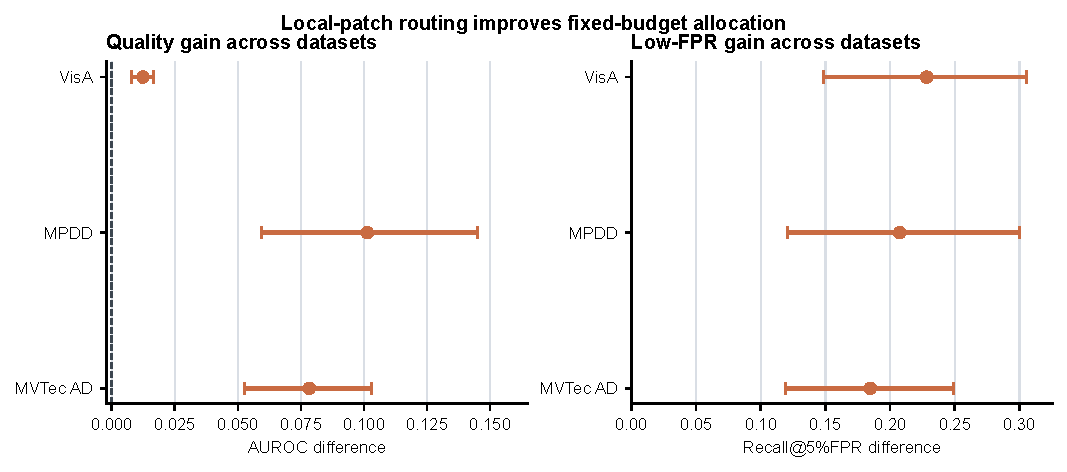
\includegraphics[width=\textwidth]{figures/Fig1_cross_dataset_effects.pdf}
\caption{Cross-dataset evidence for fixed-budget allocation. Local-patch routing minus matched-random routing is shown for image-level AUROC and Recall@5\%FPR. Points are paired differences over category--seed units and whiskers are 95\% bootstrap confidence intervals. The figure-level claim is that the allocation benefit is positive across all three datasets, while its magnitude is heterogeneous.}\label{fig:cross-effects}
\end{figure}

The full detector remains the accuracy reference. On MVTec, its pooled image-level AUROC was 0.9390. The strict 25\% local-patch and matched-random routes averaged 0.7758 and 0.6975. Thus, the local route improves allocation quality under a fixed budget, but it does not match the accuracy obtained by evaluating every image with the full detector.

The same distinction applies to the other detector references. A PaDiM-style baseline achieved pooled AUROC 0.8982 and Recall@5\%FPR 0.6544 over 45 MVTec category--seed units. A patch-level farthest-point coreset detector achieved AUROC 0.9433 and Recall@5\%FPR 0.7847 under the reported approximation. These full-budget references have higher absolute detection quality. They do not address the narrower question of whether the local route selects more useful images than matched random at the same fallback count.

\subsection{Budget sensitivity and local-score ablation}
The MVTec budget sweep remained positive at 10\%, 25\% and 50\% quotas (Table~\ref{tab:budget}). The 10\% and 50\% results were also evaluated with three seeds; their effects were +0.0511 and +0.1122 AUROC, respectively. Recall gains were +0.2853 and +0.1615. The positive differences are not confined to one quota. AUROC and low-FPR recall do not, however, change in the same way as the budget changes.

\begin{table}[t]
\caption{MVTec strict-quota budget sensitivity over 15 categories and three seeds.}\label{tab:budget}
\begin{tabular}{@{}lrrrr@{}}
\toprule
Fallback budget & AUROC $\Delta$ & Positive AUROC units & Recall $\Delta$ & Positive Recall units\\
\midrule
10\% & +0.0511 & 38/45 & +0.2853 & 40/45\\
25\% & +0.0783 & 35/45 & +0.1848 & 39/45\\
50\% & +0.1122 & 37/45 & +0.1615 & 38/45\\
\botrule
\end{tabular}
\end{table}

\begin{figure}[t]
\centering
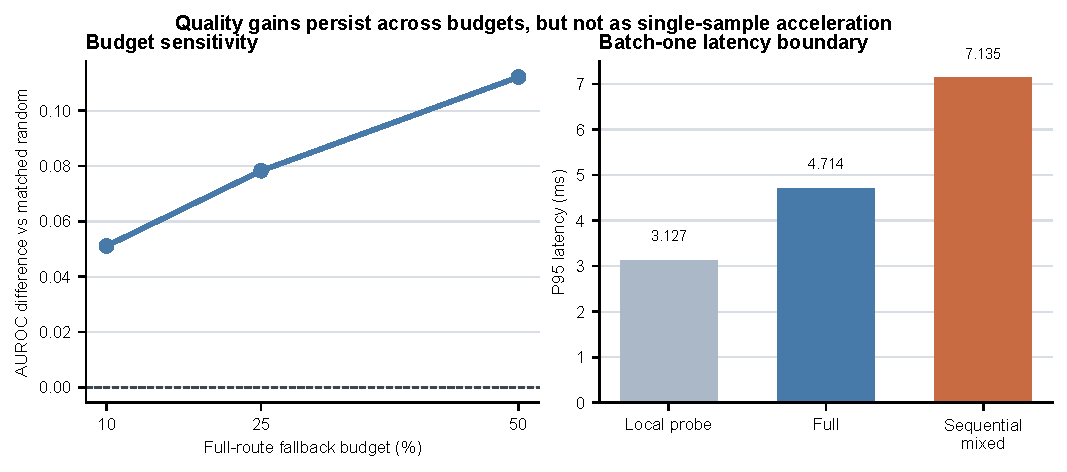
\includegraphics[width=\textwidth]{figures/Fig2_budget_latency_boundary.pdf}
\caption{Budget sensitivity and latency boundary. The left panel shows AUROC differences at strict 10\%, 25\% and 50\% fallback budgets on MVTec over three seeds. The right panel shows synchronized batch-one P95 latency for the local probe, Full detector and sequential mixed route. The quality gain persists across budgets, but the sequential route does not provide single-sample P95 acceleration.}\label{fig:budget-latency}
\end{figure}

Changing the aggregation fraction from 1\% to 5\% to 10\% on MVTec seed 17 produced AUROC differences of +0.0781, +0.0764 and +0.0830 over matched random routing. Because the differences were close and the 5\% value was fixed before the formal comparison, we retain 5\% as the main setting rather than selecting the largest value post hoc. On MPDD seed 17, the corresponding 5\% and 10\% differences were +0.1175 and +0.0823, illustrating that the best aggregation fraction is not universal.

\subsection{Failure cases and online sensitivity}
We retain the failure cases. A multi-scale rank-fusion variant underperformed matched random in a three-category MVTec smoke test and was not used in the main method. A lightweight cost-filter baseline underperformed the patch-coreset reference. The results do not support a generic benefit from adding any inexpensive score. The observed gain depends on the local-patch risk signal and the matched control.

The online prefix controller maintained an average realized fallback rate of 25.34\% on 45 MVTec category--seed units and improved AUROC by +0.0331 (95\% CI [0.0045, 0.0601]) over matched random. However, the external online audit was sensitive to dataset and buffer configuration. MPDD seed 17 showed AUROC/Recall gains of +0.0890/+0.0643, whereas VisA seed 17 showed +0.00004/-0.0408. Increasing the VisA buffer to 128 restored a positive Recall difference of +0.0750 (95\% CI [0.0189, 0.1317]) but did not produce a reliable AUROC gain (+0.00124, CI [-0.00113, 0.00339]). We therefore describe online routing as configuration-sensitive, not universally robust.

\begin{figure}[t]
\centering
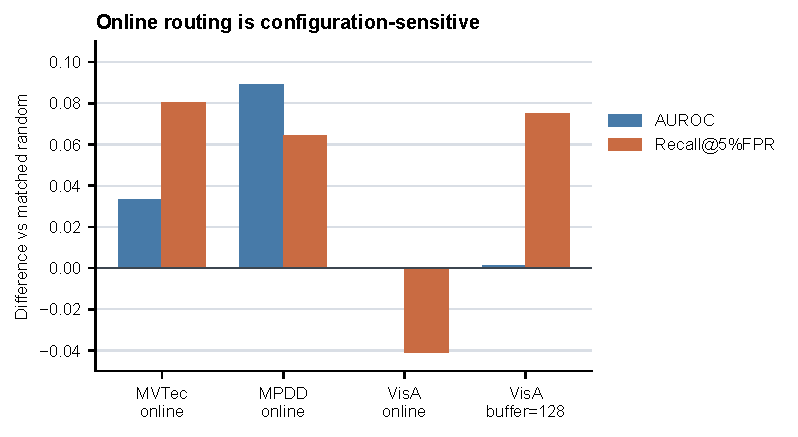
\includegraphics[width=0.85\textwidth]{figures/Fig3_online_sensitivity.pdf}
\caption{Online routing sensitivity. AUROC and Recall@5\%FPR differences from matched random are shown for the MVTec and MPDD online audits, the VisA batch-32 audit and the VisA buffer-128 sensitivity. The negative VisA batch-32 recall result and the near-zero AUROC gains bound any claim of dataset-independent online superiority.}\label{fig:online}
\end{figure}

\subsection{Latency boundary}
The synchronized batch-one CUDA audit measured P50/P95 latencies of 2.384/3.127 ms for the local probe, 4.714 ms P95 for the full detector, and 7.135 ms P95 for the sequential probe-plus-full route. The sequential route therefore does not support a single-sample P95 acceleration claim. A batch audit over three MVTec categories found lower per-image cost for the mixed route at batch 32. This is only a throughput extension and does not change the batch-one result. The result should be read as a quality improvement under a fixed allocation, not as a general latency reduction.

\section{Discussion}\label{sec:discussion}

When the number of expensive local evaluations is fixed, local-patch ranking can allocate them more effectively than random selection. This result comes from matched controls, three industrial datasets, three seeds and a budget sweep. The effect is smaller on VisA, and online routing loses low-FPR recall in some configurations.

This is not a claim that the route surpasses PatchCore or the full local path. Full-budget references remain more accurate because they evaluate every image with the expensive feature path. The contribution is the separation of detector quality from allocation quality. That distinction matters when only a fixed number of images can be escalated, but it also limits deployment claims.

There are four main limitations. Batch-one sequential P95 latency is worse than Full because the probe runs before selected samples enter the full path. Online behavior depends on batch composition, score shift and buffer size. The patch-coreset implementation is a controlled approximation of the standard reduction procedure, and learned uncertainty gatekeepers were not included as fully matched baselines. Finally, the formal evaluation uses established public benchmarks rather than the newly released ISP-AD screen-printing benchmark, which contains weakly contrasted defects and imperfect production imaging conditions \cite{krassnig2026isp}. The statistical unit is category--seed, so category-level counts should not be treated as independent evidence for every industrial class.

Future experiments should test shared feature computation, an independently trained uncertainty model and full-category deployment audits under a pre-registered P95 budget. Shift-aware calibration should control both the allocation rate and low-FPR recall. These tests would show whether the allocation effect persists after the feature path and deployment protocol change.

\section{Conclusion}\label{sec:conclusion}

A local-patch risk probe improved anomaly-detection quality over matched random escalation when the Full fallback budget was fixed at 10\%, 25\% or 50\% on MVTec and at 25\% on MPDD and VisA. The result is a quality and budget trade-off, not a general speedup. The full detector remains more accurate, batch-one P95 latency is not reduced, and online gains depend on configuration. These limits define the scope of the result.

\section{Methods}\label{sec:methods}

\subsection{Implementation details}
All experiments use ImageNet-pretrained ResNet-18 features. The fast path uses $128\times128$ inputs and layer-2 features; the full path uses $224\times224$ inputs and layer-3 patch features. Normal training images only are used to construct memory banks. The main local probe uses the top 5\% aggregation fraction. Seeds 17, 29 and 41 are fixed across the formal experiments. The evaluation code records category, seed, budget, realized fallback rate, AUROC, Recall@5\%FPR and latency fields in JSON output.

\subsection{Latency measurement}
Latency was measured on CUDA with explicit synchronization, one warm-up and repeated cached-image evaluation. P50 and P95 values are reported for the local probe, Full path and sequential mixed path. Timing repetitions are treated as repeated measurements of a system property and are not used as independent units in the accuracy bootstrap.

\subsection{Statistical analysis}
For each dataset and budget, the paired comparison is formed at the category--seed level. Bootstrap resampling samples these units with replacement and computes the route difference for each replicate. We report two-sided 95\% confidence intervals. The primary inference is based on whether the interval for the paired difference excludes zero and on the direction and magnitude of the effect; category-level positive counts are descriptive.

\subsection{Ethics and reproducibility}
This study uses public image datasets and does not involve human participants, animals or personally identifiable information. Public dataset sources are cited in the reference list. The split protocol, source data for the figures, derived result tables and evaluation scripts are available at \url{https://github.com/cdhuangjin/fixed-budget-patch-routing}.

\backmatter

\section*{Acknowledgements}
The authors thank the maintainers of MVTec AD, MPDD and VisA for making the benchmark datasets available.

\section*{Declarations}
\textbf{Funding.} No funding was received for conducting this study or preparing the manuscript.

\textbf{Competing interests.} The authors declare no relevant financial or non-financial competing interests.

\textbf{Ethics approval and consent to participate.} Not applicable; the study uses public benchmark datasets and does not involve human or animal participants.

\textbf{Consent for publication.} Not applicable.

\textbf{Data availability.} MVTec AD, MPDD and VisA are publicly available benchmark datasets. The derived category--seed result tables and figure source data are available at \url{https://github.com/cdhuangjin/fixed-budget-patch-routing}.

\textbf{Code availability.} The evaluation scripts, configuration files and route definitions are available at \url{https://github.com/cdhuangjin/fixed-budget-patch-routing}.

\textbf{Author contributions.} J.H. designed the study, implemented the analysis, performed the experiments and drafted the manuscript. Q.G. contributed to experimental review, interpretation and manuscript revision. Both authors approved the final manuscript.

\bibliography{references}

\end{document}
